\section{Introduction}
\label{sec:intro}

As one of the foundation for safety in autonomous driving, many research efforts in lane detection focus on making detection model accurate and robust.
Over the past few years, 2D lane detection methods have shown impressive performances~\cite{jin2022eigenlanes, hou2019learning, liu2021end, wang2022keypoint, huang2023anchor3dlane}.
However, due to the lack of depth information, transforming 2D images to 3D space still remains highly challenging.
Recently, large-scale datasets with 3D lane annotations have been proposed.
This has been promoted the research of 3d lane line representation and detection~\cite{chen2022persformer, efrat20203d, garnett20193d, guo2020gen, liu2022learning, yan2022once, huang2023anchor3dlane}.
Compared to 2D lane, 3D lane detection can directly obtain the slope information of the lane, to help autonomous vehicles make better decisions.
%3D Lane Detection is critical for various applications in autonomous driving, such as trajectory planning and lane keeping.
%Despite the remarkable progress of LiDAR-based methods in other 3D perception tasks~\cite{zhou2018voxelnet, lang2019pointpillars},
%recent advances in 3D lane detection prefer using a monocular camera since it owns desirable advantages compared to LiDARs.


\begin{figure}[ht]
    \centering
    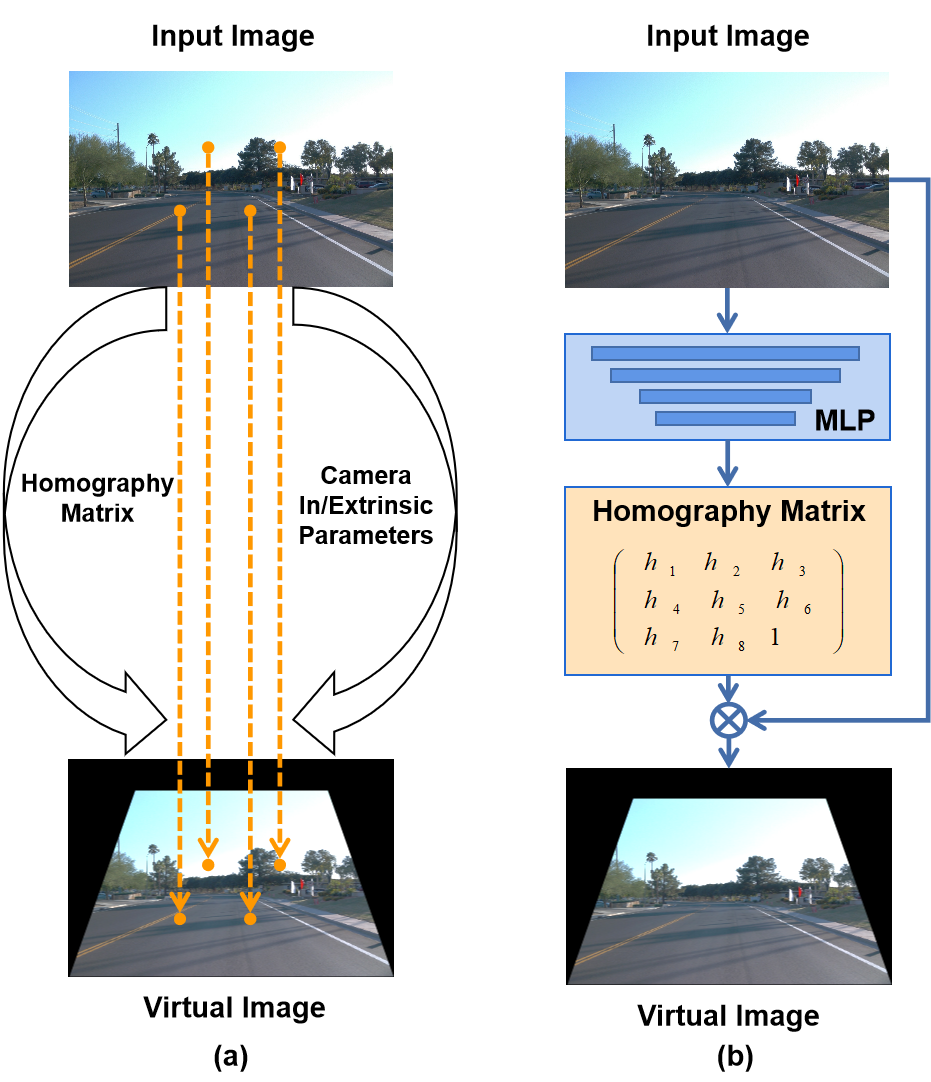
\includegraphics[width=0.8\linewidth]{asset/fvhnet}
    \caption{(a) Fixed parameters transformation matrix, which based on camera in/external parameters.
        (b) MLP-based transformation matrix, which learns a perspective transformation conditioned on the input image.}
    \label{fig:intro}
\end{figure}

Among these methods for 3D lane line detection, BEV-based methods~\cite{chen2022persformer, efrat20203d, guo2020gen, liu2022learning, wang2023bev} have received attention from researchers due to the accuracy, robustness, and speed.
These methods need a spatial transformation module to transform front-view features to bev-view.
In Bev-LaneDet\cite{wang2023bev}, spatial transformation module is fixed spatial mapping by MLP,
which are difficult to be integrated with the camera in/extrinsic parameters, resulting in poor performance.
To address this issue, it realizes a preprocessing method of quickly
unifying the camera in/extrinsic parameters by establishing
a Virtual Camera with standard in/extrinsic parameters, which are fixed parameters derived from the mean value of the in/extrinsic
parameters of the training dataset.
However, different cameras mounted on the vehicle have different internal/external parameters, which have a significant effect on features transformation and 3D lane results.
As illustrated in Fig.\ref{fig:intro}(a)\@, if a fixed transformation matrix is employed to get homography matrix for features transformation, the projection becomes less accurate.
Therefore, we need unify the in/extrinsic parameters of front-facing cameras on different vehicles.

Towards this issue, we proposed a MLP-based homography matrix estimation network,
called \textbf{F}ront-\textbf{V}irtual \textbf{H}omograph Matrix Net, which makes homography matrix learnable instead of fixed.
As show in Fig.\ref{fig:intro}(b)\@. FVHNet takes the RGB image as input and predicts the parameters to generate the homography matrix.
We project the input images to the virtual camera by multiplying the homography matrix.
After this transformation, we input the virtual-view image features to backbone network which output the front-view features.
Then, we can get the 2d prediction by a front-view lane detection head.
Finally, the front-view prediction is re-projected back to the original image space by multiplying the inverse homography matrix
and compute the loss between the prediction and ground truth.
Through this way, the model can be trained effectively without providing any extra annotations except for the original lane labels.


\textbf{In general, our main contributions are three-fold:}
% hzm----
%\textbf{1)} We propose to extract homographic parameters from input image by MLP networks, making homography matrix learnable.
%With a more accurate homographic matrix, in/extrinsic can be unified in a more robust virtual camera. We propose to extract homographic parameters from input image by MLP networks, making homography matrix learnable.
\textbf{1)} FVHNet, a MLP-based network that can learn transformation matrix parameters which can transform input images to virtual camera images.
\textbf{2)} FVHLoss, a loss function to supervise FVHNet training, which only needs the annotations of lane marks.
%\textbf{3)} We conducted experiments on both real and synthetic datasets, This method shows remarkable detection accuracy on both the OpenLane and Apollo Synthetic datasets;
\textbf{3)} Our method is validated on the Apollo 3D synthetic dataset, achieving the promising performance. %compared with